\section{Cancelaci�n}
%TODO: hacer los diagramas por el amor de Dios
La cancelaci�n es un evento que involucra tanto al componente cocina como al componente de pedidos fuera de la cocina, por lo que podria incluso considerarse un componente separado. 

Mediante la interfaz grafica se selecciona un pedido y se invoca el metodo cancelar que posee el mismo, este metodo lo que hace es invocar el cancelar del responsable de cancelacion del pedido. Decidimos hacerlo de esta manera, en primer lugar, porque la cancelaci�n es un proceso que puede ser complejo, ya que por ejemplo, al cancelar un pedido que estaba en el horno, hay que avisar al maestro de que saque ese pedido, porque no hay que seguir cocinando. Sacar este pedido de la cocina puede implicar seleccionar un nuevo pedido a cocinar segun la politica vigente. De manera similar, una cancelaci�n de un pedido que se esta preparando requiere avisar al maestro de la cancelaci�n, para pedirle el stock reutilizable, asi como tambi�n buscar un nuevo pedido a preparar. Por esta raz�n, nos parece acertado que aquellos que pueden llegar a tener que efectuar acciones particulares debido a una cancelaci�n, sean invocados por el pedido cuando es cancelado. Notemos que este acercamiento es considerablemente extensible, ya que si se pretende por ejemplo agregar un nuevo controlador, solo debe implementar el m�todo cancelar y asegurarse de que aquellos pedidos que quedan bajo su control lo tienen a el como responsable de cancelarlo.

Ademas de esta manera de resolver el problema consideramos otras formas que no fueron aplicadas. En primer lugar, pensamos en que el pedido de cancelaci�n ingresar por el coordinador de pedidos, el cual va propagando el llamado a todos los agentes a los que tiene acceso, para que estos se fijen si les corresponde cancelar o no. Esto tiene como principal problema que se realiza un cantidad de llamadas innecesarias, pero como caracteristica positiva tiene que es bastante distribuida, ya que si bien el llamado entra por el coordinador, las invocaciones a cancelar se propagan a todos los posibles agentes.

Otra alternativa era considerar una clase canceladora que se encargue de rastrear el pedido, y luego decirle al controlador que lo estaba manejando en ese momento que lo cancele. El problema de esto es que el cancelador para buscar al responsable, va a tener que utilizar por ejemplo que los pedidos en tal estado si son de tal tipo estan bajo la orbita de tal controlador. Esto no nos parecio correcto, ni extensible, por lo cual se descart�.

Veamos a continuaci�n algunos escenarios diferentes de cancelaci�n.

El primer escenario consiste en cancelar un pedido que estaba en la cola de ingreso. En este caso se debe sacar de dicha cola al pedido y se debe reestablecer el stock de los insumos que no se van a utilizar.

\begin{figure}[H]
\centering
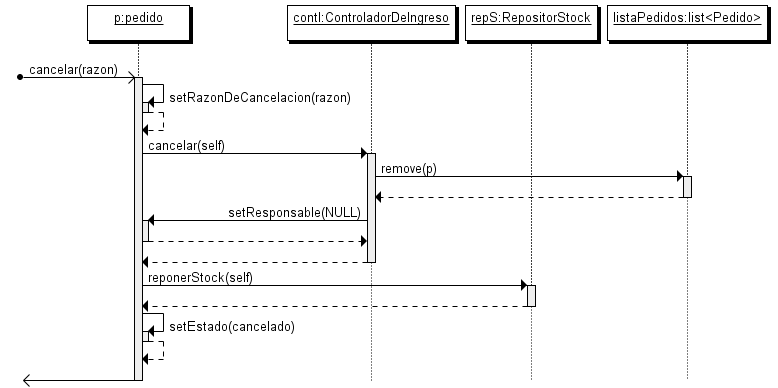
\includegraphics[height=9cm]{./figuras/cancelacionIngreso.png}
\caption{Cancelaci�n de un pedido ingresado}
\end{figure}

En segundo lugar podemos considerar que ocurre cuando se cancela un pedido que esta en preparaci�n. En este caso puede ocurrir que el pedido se estaba preparando en el momento de su cancelaci�n, por lo que debe indicarse que se detenga la preparaci�n y que se indiquen que insumos se pueden salvar.

Si la cancelaci�n se hace para un pedido que estaba en la cola nada mas, el proceso es muy simple, solo se desencola esta parte que estaba esperando y listo. El escenario mas interesante, que es el vamos a modelar ocurre cuando lo que se cancela estaba siendo preparador. Veamos entonces que pasa si un pedido que tenia sus empanadas siendo preparadas, y se cancela, asumiendo que hay otro pedido con empanadas en la cola. 

\begin{figure}[H]
\centering
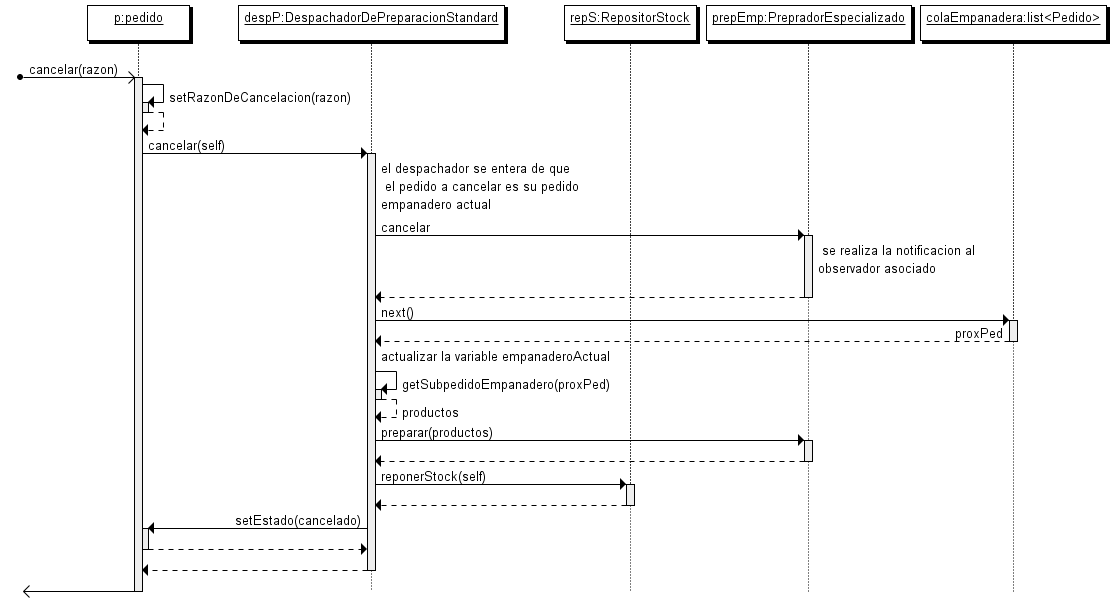
\includegraphics[height=9cm]{./figuras/cancelacionPreparacion.png}
\caption{Cancelaci�n de un pedido ingresado}
\end{figure}

Otros lugar donde la cancelaci�n es mas conflictiva es durante la coccion de un pedido, si el mismo estaba en la cola el proceso es simple porque solo hay que sacarlo de la misma. Ahora si el pedido estaba en el horno o estaba a medio cocinar hay que avisar al maestro para que deje de cocinar el pedido.

Vamos a modelar el escenario en el que el pedido que se cancela, era el pedido a medio cocinar del horno 1. Entonces hay que avisar su cancelaci�n, y buscar un nuevo pedido para poner en su lugar. Vamos a suponer tambi�n que el pedido tenia dos partes en cocci�n, que no estaban en modulos agiles y que el proximo pedido de la cola necesitaba de un mas de 2 modulos para cocinarse.

\begin{figure}[H]
\centering
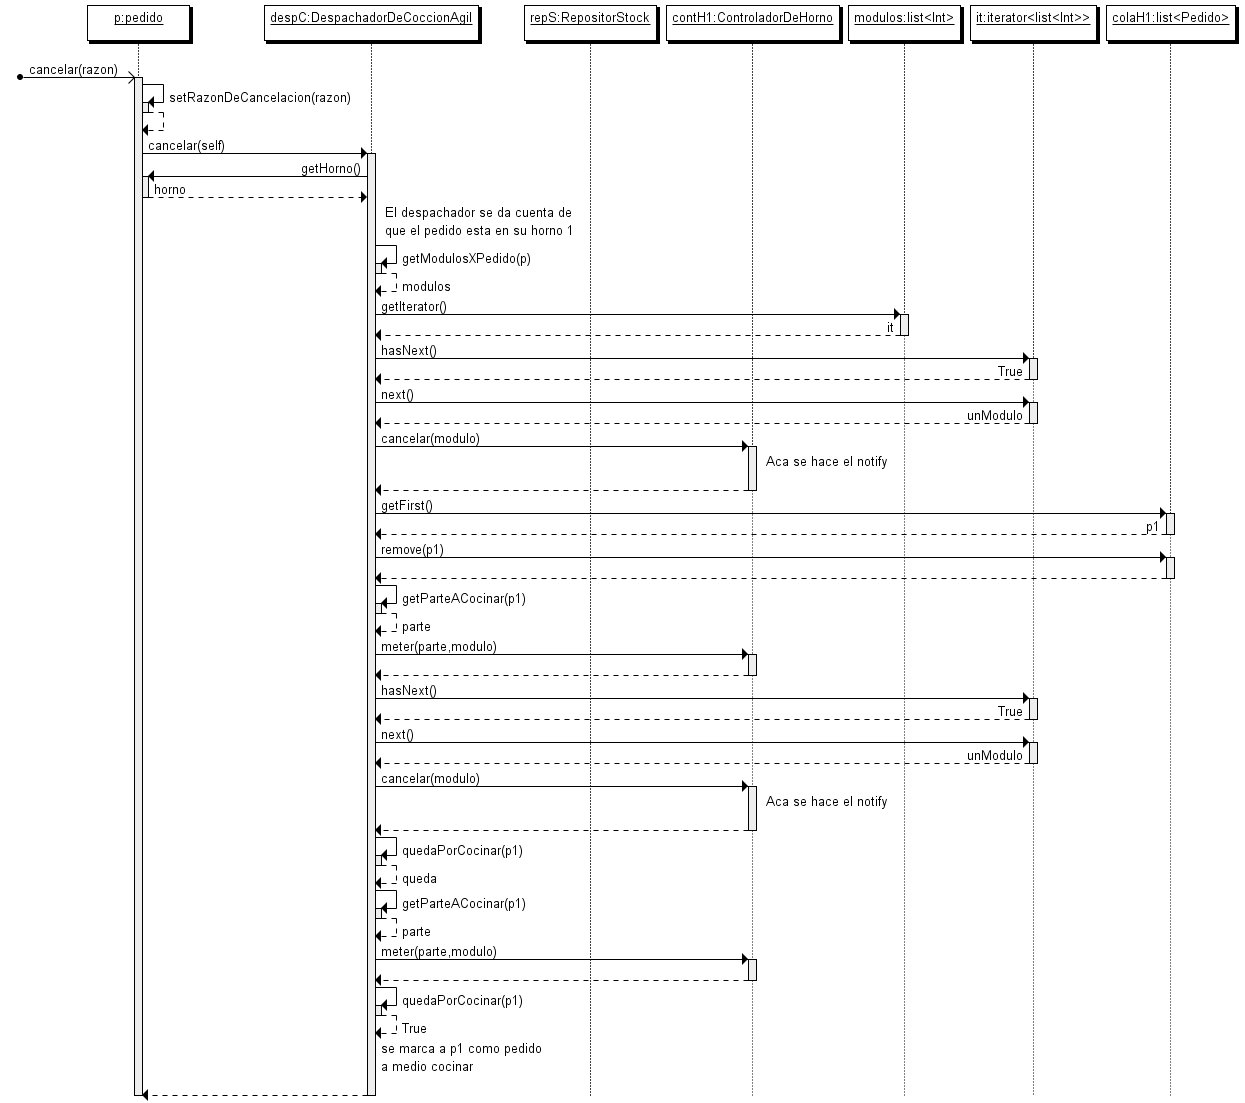
\includegraphics[height=13cm]{./figuras/cancelacionCoccion.png}
\caption{Cancelaci�n de un pedido ingresado}
\end{figure}

Mas en general podriamos variar los parametros, pero la secuencia seria similar. Es por esto que no realizaremos mas diagramas sobre la cancelaci�n en la cocina.

Finalmente la cancelaci�n tambi�n puede darse en el ambito del controlador de entregas y del controlador de listos, en estos casos el manejo es simple, sin embargo, por ejemplo en el controlador de entregas, si la operatoria no fuera de contingencia podria requerir de una logica mas compleja de aviso al delivery.

Otro aspecto importante de la cancelaci�n es la reposici�n del stock, la cual puede ser automatica o puede requerir que se indique que insumos se pudieron rescatar